% Page 032 — page imprimée 28
% Contenu seul : le préambule et la pagination sont gérés par meyrueis.tex

\sectiondate{Les chapeliers de Meyrueis}{1900}


A quelle époque avait bien pu naître la chapellerie de Meyrueis ? Sans grande précision on
peut penser que c’est du temps de Basville, lors des dragonnades, que se sont installés des
chapeliers à Meyrueis. On fabriquait de bons chapeaux de laine communs destinés aux classes
populaires.\\

\begin{itemize}
\item En 1793, 14 chapeliers payent patente
\item En 1845, 12 entreprises, 17 ateliers emploient 200 salariés. C’est l’âge d’or !!!
\item En 1900, 3 ateliers et 35 salariés
\end{itemize}

\vspace{0.5em}

Tout au long du 19\ieme siècle les chapeliers, avec les tisserands, assurèrent à la collectivité de
Meyrueis des revenus réguliers et forts appréciables permettant un débouché local à la laine,
aux bourres de soie voire peut-être aux poils de lapin pour des chapeaux fins, bourgeois ou de
« grande fabrique ».

\medskip

\textbf{La Chapellerie Couderc}

Elle fut la dernière à fonctionner avec les Etablissements Veyrier les plus importants. Nous
avons encore des copies de commandes et de factures de 1898 à 1915. Ce furent sans doute
les dernières... Les ateliers étaient installés dans deux petites maisons de la Placette côté
rivière et lorsque « l’eau venait », aux grandes crues d’automne toute la famille Couderc-
Loupiac déménageait les chapeaux, les outils et les petites machines au Ferradou à la maison
de Timberle adossée au Rocher du Château.

\vspace{0.7em}

La fabrication et le commerce portaient sur plusieurs centaines de chapeaux, sans doute 2000 à
3000 par an et peut-être beaucoup plus puisqu’on trouve des commandes de plusieurs
centaines de cloches voire 1000 d’un coup à Espéraza ou à Chalabre dans l’Aude. Les
chapeaux étaient terminés à Pont Vieux, mis en forme, avec les garnitures en cuir, les galons,
le repassage et le lustrage voire l’imperméabilisation puisqu’en 1911 Auguste écrit à une de ses clientes : « ... j’ai fait récemment breveter un procédé pour faire des chapeaux que la pluie
ne traverse pas ». Très vite ces chapeaux imperméables représenteront 75\% de la production.

% Page 033 — page imprimée 29
% Contenu seul : le préambule et la pagination sont gérés par meyrueis.tex

Le nombre d’ouvriers devait être réduit . Aucune pièce en notre possession n’y fait allusion.
Mais nous venons de retrouver aux Archives un recensement énigmatique :
En 1883 avait été recensé un foulon de feutre pour les chapeaux.
De 1884 à 1895 la chapellerie était taxée pour 3 ouvriers mais une note indique 2 ouvriers
foulonniers, 3 fabricants, 3 ouvriers finisseurs. Alors qu’en penser ?

Nous voyons seulement qu’Auguste avait en charge toute la partie commerciale et le courrier
avec les fournisseurs et les clients. Un de ses fils Albert visitait les clients comme voyageur de
commerce après avoir été représentant, en 1911, chez un chapelier de Paris (maison Kohn et
Levy) 125 rue du Faubourg Montmartre. Son père Auguste le recommande à plusieurs
reprises à certains de ses clients pour qu’ils l’embauchent comme stagiaire ou représentant ?
Auguste commande des cloches en mérinos ou cashmere, des feutres avec des poils de lapin
qu’on ne peut teindre qu’avec des produits spéciaux surtout au moment de Pâques où les
commandes sont nombreuses.
Mais en ces années d’avant-guerre il se plaint « de la hausse constante des matières premières
et du prix de la main d’œuvre toujours plus élevé ».

La plupart des opérations se faisaient à la main mais déjà apparaissent des machines : par
exemple en 1903 « j’ai perfectionné l’outillage destiné à faire la tournure aux chapeaux ;
vous reconnaîtrez la différence... » en 1908 « une passeuse et ses accessoires actionnée par
une machine à vapeur. » que l’on revendra en 1913 en Algérie pour en acheter une plus
moderne. On est en relation avec Thimonnier à Lyon, (un célèbre fabricant d’aiguilles et de
machines). Il est question d’une machine Gutzner puis d’une Selecta avec leurs accessoires.
D’où avant la guerre de 1914 une certaine mécanisation de la production.

\textbf{On ne faisait quand même pas fortune :} ainsi Auguste écrit au sous préfet de Florac en
1911 pour lui demander une réduction d’impôts « ...nous avons un locataire pendant un mois
d’été et pendant ce temps nous faisons la cuisine sous un hangar et notre chambre est au
galetas sur des tréteaux... »
En 1912 c’est au Préfet qu’il s’adresse pour lui demander une réduction de sa patente : « ...les
commerces deviennent plus nombreux et plus importants sur la place centrale de Meyrueis et
il y a moins de monde à Pont Vieux... »

Auguste et ses enfants continuent toujours à s’occuper de la propriété et on vit beaucoup sur
les pommes de terre et les légumes du jardin, les châtaignes de Cabanals, les lapins ou le
cochon. Ainsi on achète 300 choux à repiquer et en même temps trois livres de truites.
La machine à vapeur est alimentée par le charbon de Lanuejols (20 à 30 quintaux) venant de
la mine des Gardies livré par Causse dit Carrot, roulier à Lanuejols.

On achète à l’extérieur mais on vend aussi quand l’occasion se présente :

« ... Quand vous aurez du vin, envoyez moi une barrique, du bon... » 1903

« ... A la dernière foire mon père est sorti pour acheter le cochon... »

« Je vous envoie 6 doubles de châtaignes et une grillade pour vous. Elles sont très jolies,
plus que d’habitude car j’ai taillé tous les arbres de petite espèce pour les greffer. Si vous en
avez la vente je peux vous envoyer une autre sac ou deux... » 25 oct. 1902 à Blanc du Rozier.

% Page 034 — page imprimée 30
% Contenu seul : le préambule et la pagination sont gérés par meyrueis.tex

« ...Pour les tourdres, je le regrette bien mais jusqu’ici il est impossible d’en trouver, la
surveillance est si sévère que les paysans n’osent pas s’aventurer. On parle de 6 mois de
prison et de 500 ou 600 F. d’amende. Si, un peu plus tard, je peux en trouver quelques uns soyez
assuré que je ferai mon possible mais je ne puis rien vous promettre. » M. Gasc à Requista

\medskip

\textbf{La guerre de 1914-18}

Sur le plan politique les menaces s’accumulent et l’on entend des bruits de botte. Fin 1912
Albert est convoqué pour une période d’instruction militaire. Dix-huit mois plus tard ce sera la
guerre, et Albert sera tué lors de la bataille de Soissons.

Son père comptait sur lui pour reprendre et relancer la chapellerie après la disparition de Paul,
l’aîné.

\medskip

Que lui était-il donc arrivé ?

Dans les années 90 Paul était tombé amoureux fou d’une de ses cousines germaines Emma,
fille de Louis . Elle l’aimait bien et l’appréciait comme cousin mais pas plus et elle ne lui
laissa aucun espoir.

Paul en fut terriblement affecté et lorsque l’occasion s’en présenta (?) il partit pour le Chili
pour oublier et probablement aussi pour prendre des contacts pour un éventuel commerce de
chapeaux avec ce pays. Muni d’un petit pécule il embarqua sur un vapeur pour Santiago et...
« on n’eut plus jamais aucune nouvelle de lui. » Est-il mort de maladie ? A-t-il été assassiné ?
Nul ne le sait. C’est là la tradition Loupiac. A Cambonéral chez les Verdier la mémoire est
restée plus vive : « Il nous a toujours été raconté que Paul s’était embauché dans une
chapellerie au Chili. Il avait été happé par une machine et en serait mort. » On peut penser
que Léonie sœur cadette de Paul Couderc donnera à son fils en souvenir de son frère disparu
le même prénom afin de ne pas l’oublier...

Les deux fils disparus, Auguste se retrouvait seul avec ses deux filles (Marie infirme et
célibataire et Marthe qui mourra d’un cancer à Montpellier en 1925, célibataire elle aussi)
pour continuer la chapellerie mais il avait 74 ans. La guerre continuait avec son cortège de
morts. Découragé et fatigué il arrêta la fabrication et ferma la chapellerie à peu près au même
moment que les établissements Veyrier pourtant beaucoup plus importants.

On ne parlera plus désormais des chapeliers de Meyrueis.

La guerre cette « maudite guerre » comme avait dit son frère Louis avait disloqué beaucoup
de familles de la campagne, laissant des veuves et des filles qui ne se marièrent pas car des
millions de jeunes hommes avaient été massacrés. Dès lors avec la modernisation, les petites
filatures, les tissages et les chapelleries de notre ville de Meyrueis étaient condamnés. Et qui
peut comprendre la souffrance des survivants ?

% Page 035 — page imprimée 31
% Contenu seul : le préambule et la pagination sont gérés par meyrueis.tex


Le chapeau fabriqué à Meyrueis était un feutre de laine teint en
noir, à larges bords le plus souvent souples. Tantôt sa coiffe
était ronde, en feutre mou mais résistant, tantôt elle avait
l’allure d’un cône évasé relativement haut.

On distingue deux catégories de chapeaux :

\begin{itemize}
\item Le feutre souple à larges bords, fabriqué manuellement
protégeant avantageusement le front, le cou et le visage (N° 2,
3, 4, 5 et 6), traditionnellement porté pour les travaux des
champs.

\item La deuxième catégorie (1, 7, et 8) concerne une seconde
génération de chapeaux plus spécialement confectionnés
pendant la période de mécanisation des ateliers : un galon de
même couleur que le feutre ajoute une note d’élégance... C’est
le chapeau Couderc de 1910, Un secret de fabrication, breveté
le rendait imperméable.
\end{itemize}

\begin{center}
\textit{(D’après un article de Jean Claude Crespin)}
\end{center}

\begin{center}
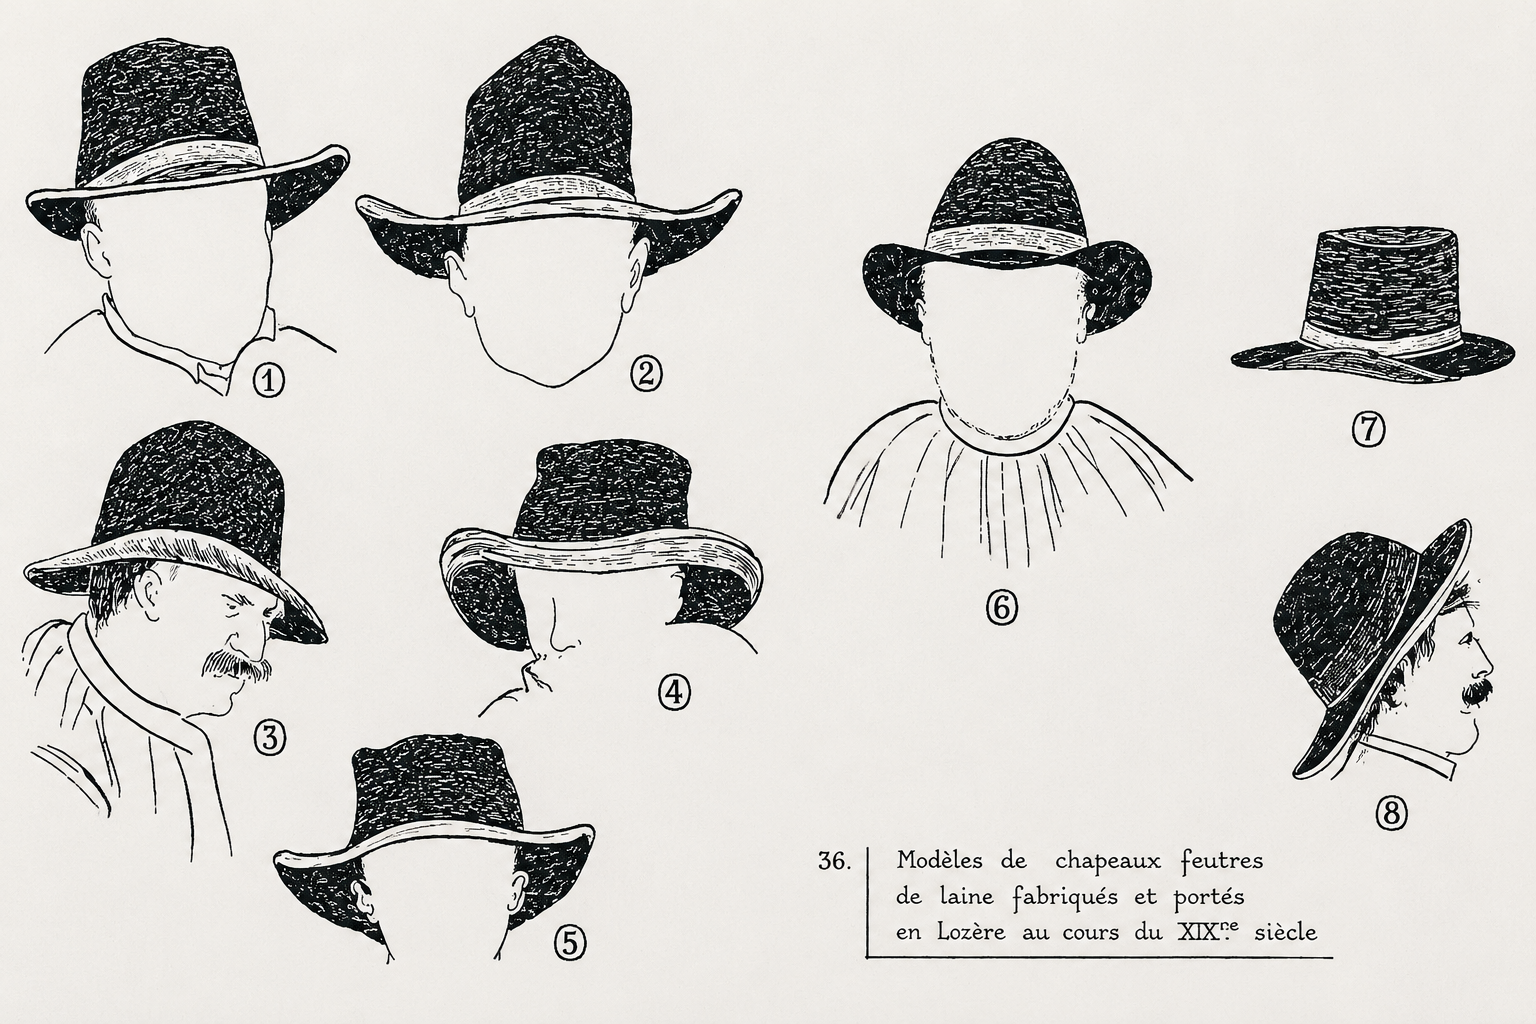
\includegraphics[width=\textwidth]{imgs/035.png}
\end{center}
